\section{Date: 2026-10-31}
\noindent \textbf{Series ID: ADPMCDMANERNSA} 

\noindent This series is titled Nonfarm Private Employment in the Middle Atlantic Census Division and has a frequency of Monthly. The units are Persons and the seasonal adjustment is Not Seasonally Adjusted.The observation start date is 2010-01-01 and the observation end date is 2026-09-01.The popularity of this series is 1. \\ 

\noindent \textbf{Series ID: CIU2010000100000I} 

\noindent This series is titled Employment Cost Index: Total compensation for Private industry workers in Management, professional, and related and has a frequency of Quarterly. The units are Index Dec 2005=100 and the seasonal adjustment is Not Seasonally Adjusted.The observation start date is 2001-01-01 and the observation end date is 2026-07-01.The popularity of this series is 15. \\ 

\subsection{Raw Regression}
\noindent Regresses the two series against each other directly. A significant result here can come just as easily from both series sharing a long-run trend as from any real relationship.

\begin{center}
\begin{tabular}{lclc}
\toprule
\textbf{Dep. Variable:}              & value\_fred\_CIU2010000100000I & \textbf{  R-squared:         } &     0.769   \\
\textbf{Model:}                      &              OLS               & \textbf{  Adj. R-squared:    } &     0.765   \\
\textbf{Method:}                     &         Least Squares          & \textbf{  F-statistic:       } &     216.4   \\
\textbf{Date:}                       &        Sat, 31 Oct 2026        & \textbf{  Prob (F-statistic):} &  2.33e-22   \\
\textbf{Time:}                       &            16:24:36            & \textbf{  Log-Likelihood:    } &   -237.92   \\
\textbf{No. Observations:}           &                 67             & \textbf{  AIC:               } &     479.8   \\
\textbf{Df Residuals:}               &                 65             & \textbf{  BIC:               } &     484.2   \\
\textbf{Df Model:}                   &                  1             & \textbf{                     } &             \\
\textbf{Covariance Type:}            &           nonrobust            & \textbf{                     } &             \\
\bottomrule
\end{tabular}
\begin{tabular}{lcccccc}
                                     & \textbf{coef} & \textbf{std err} & \textbf{t} & \textbf{P$> |$t$|$} & \textbf{[0.025} & \textbf{0.975]}  \\
\midrule
\textbf{const}                       &    -153.4786  &       19.702     &    -7.790  &         0.000        &     -192.827    &     -114.130     \\
\textbf{value\_fred\_ADPMCDMANERNSA} &    1.793e-05  &     1.22e-06     &    14.709  &         0.000        &     1.55e-05    &     2.04e-05     \\
\bottomrule
\end{tabular}
\begin{tabular}{lclc}
\textbf{Omnibus:}       &  3.428 & \textbf{  Durbin-Watson:     } &    0.417  \\
\textbf{Prob(Omnibus):} &  0.180 & \textbf{  Jarque-Bera (JB):  } &    2.519  \\
\textbf{Skew:}          &  0.319 & \textbf{  Prob(JB):          } &    0.284  \\
\textbf{Kurtosis:}      &  2.297 & \textbf{  Cond. No.          } & 3.04e+08  \\
\bottomrule
\end{tabular}
%\caption{OLS Regression Results}
\end{center}

Notes: \newline
 [1] Standard Errors assume that the covariance matrix of the errors is correctly specified. \newline
 [2] The condition number is large, 3.04e+08. This might indicate that there are \newline
 strong multicollinearity or other numerical problems.

\begin{figure}
\centering
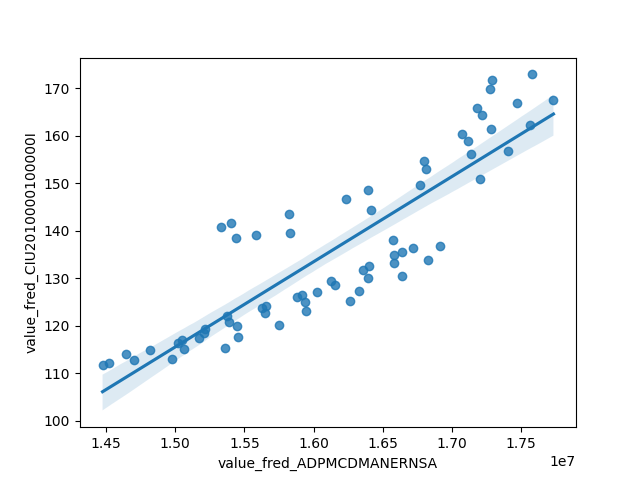
\includegraphics[scale = 0.9]{plots/plot_2026-10-31.png}
\caption{Raw Regression Plot for 2026-10-31}
\end{figure}
\newpage
\subsection{Detrended Regression}
\noindent Regresses the residuals of each series after removing its own linear time trend, so a shared trend can no longer drive the result on its own. A relationship that stays significant here is better evidence of a genuine link between the two series.

\begin{center}
\begin{tabular}{lclc}
\toprule
\textbf{Dep. Variable:}                         & value\_fred\_CIU2010000100000I\_detrended & \textbf{  R-squared:         } &     0.009   \\
\textbf{Model:}                                 &                    OLS                    & \textbf{  Adj. R-squared:    } &    -0.006   \\
\textbf{Method:}                                &               Least Squares               & \textbf{  F-statistic:       } &    0.5914   \\
\textbf{Date:}                                  &              Sat, 31 Oct 2026             & \textbf{  Prob (F-statistic):} &    0.445    \\
\textbf{Time:}                                  &                  16:24:37                 & \textbf{  Log-Likelihood:    } &   -178.49   \\
\textbf{No. Observations:}                      &                       67                  & \textbf{  AIC:               } &     361.0   \\
\textbf{Df Residuals:}                          &                       65                  & \textbf{  BIC:               } &     365.4   \\
\textbf{Df Model:}                              &                        1                  & \textbf{                     } &             \\
\textbf{Covariance Type:}                       &                 nonrobust                 & \textbf{                     } &             \\
\bottomrule
\end{tabular}
\begin{tabular}{lcccccc}
                                                & \textbf{coef} & \textbf{std err} & \textbf{t} & \textbf{P$> |$t$|$} & \textbf{[0.025} & \textbf{0.975]}  \\
\midrule
\textbf{const}                                  &    1.132e-12  &        0.431     &  2.63e-12  &         1.000        &       -0.860    &        0.860     \\
\textbf{value\_fred\_ADPMCDMANERNSA\_detrended} &    8.324e-07  &     1.08e-06     &     0.769  &         0.445        &    -1.33e-06    &     2.99e-06     \\
\bottomrule
\end{tabular}
\begin{tabular}{lclc}
\textbf{Omnibus:}       & 11.990 & \textbf{  Durbin-Watson:     } &    0.036  \\
\textbf{Prob(Omnibus):} &  0.002 & \textbf{  Jarque-Bera (JB):  } &    4.477  \\
\textbf{Skew:}          &  0.343 & \textbf{  Prob(JB):          } &    0.107  \\
\textbf{Kurtosis:}      &  1.936 & \textbf{  Cond. No.          } & 3.98e+05  \\
\bottomrule
\end{tabular}
%\caption{OLS Regression Results}
\end{center}

Notes: \newline
 [1] Standard Errors assume that the covariance matrix of the errors is correctly specified. \newline
 [2] The condition number is large, 3.98e+05. This might indicate that there are \newline
 strong multicollinearity or other numerical problems.

\begin{figure}
\centering
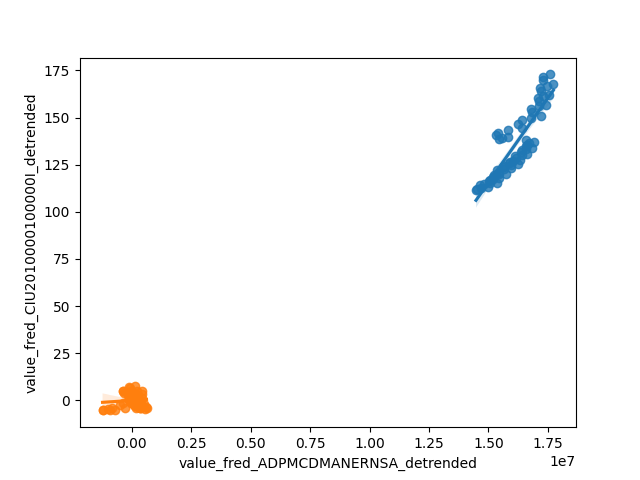
\includegraphics[scale = 0.9]{plots/plot_2026-10-31_detrended.png}
\caption{Detrended Regression Plot for 2026-10-31}
\end{figure}
\newpage
